Paper's authors conducted attacks in the digital domain (Sec 8.1) and in physical world (Sec 8.2).

\subsection{Digital-Environment Experiments}

Digital environment attacks assumes that attacker has access to FRS input system and can manipulate input images on a pixel level, so we don't need to care about physical-realizability (See Sec. 7). Our only concern is minimizing \textit{softmaxloss} (See Sec. 6.3). Intuitively this kind of attacks should be easier to conduct. 

Sharif et. al ran 8 different attacks (See Figure 15) on the DNNs described in Sec. 5. The experiments differed in the purpose of the attack, the type of perturbation (the whole face or just eyeglass frames) and the type of attacked DNN ($DNN_A$ $DNN_B$ or $DNN_C$, see Sec. 5)

The success rate was measured as a percentage (success rate) of attacks in which attacker was recognized as target $t$ (for impersonation attacks) or not recognized as himself/herself. For each attack Sharif et. al used 10 or 20 different attackers, 3 images for each attacker and reported mean success rate for those images.

The obtained results were impressive. In experiments 1 and 2 (in which attacker could change any pixel at the face) conducted attacks had 100\% success rate. However changes in pixel values were very small, imperceptible to humans and not very practical. Perturbations are smaller then camera sampling error so it would be not possible to use such image to conduct successful attack on FRS in the physical world. 

Experiments 3-8 used perturbation in a eyeglass frames shape, here results were also quite impressive. For all of dodging experiments (3-5) success rate was 100\%. The only attack that have slightly worst performance result was impersonation attack on $DNN_A$. Here success rate was below 92\%, which might be caused by big number of classes. The obtained results suggest that impersonation attacks are more difficult to perform then dodging attacks.

\begin{figure}[!ht]
  \centering
  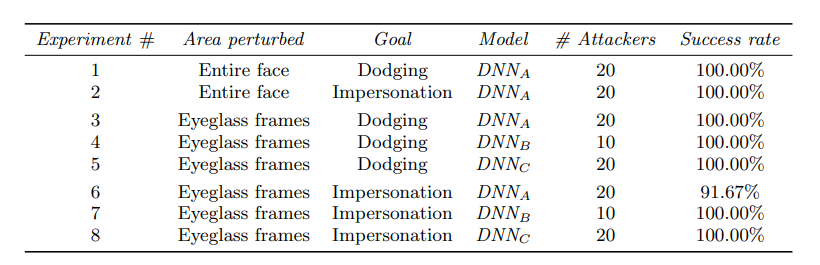
\includegraphics[scale=0.7]{Images/digital-env-experiments.png}
  \caption{Attack results in digital environment [2]}
  \label{figurelabel}
\end{figure}

\subsection{Physical-Realizability Experiments}

As mentioned in Sec. 7 \textit{Successful attack in digital environment does not guarantee same success in a physical world}. In physical wold we have to deal with camera sampling errors or printing limitations and as a result we have to modify the objective which we use to find perturbation (See equation 10). 

For physical-realizability Experiments Sharif et. al ran 6 different attacks (See Figure 16) on the $DNN_B$ and $DNN_C$. To take pictures authors used Canon T4i camera, eyeglass frames were printed with an Epson XP-830 printer on Epson Glossy photo paper. $\kappa_1$ and $\kappa_2$ hyper-parameters were set to $0.15$ and $0.25$ respectively. As as attacker authors have used themselves, the targets to attack were randomly selected. 

For each subject they collected about 30-50 photos in each of five sessions. First session was used to collect set $X$ of images of attackers not wearing any eyeglass frames. This set $X$ was later used for generating perturbation eyeglass frames, used later in the attacks. Session 2 and 3 were used to conduct dodging attacks on $DNN_B$ and $DNN_C$, Sessions 4 and 5 were used to conduct impersonation attacks  on $DNN_B$ and $DNN_C$.

All 3 attacker succeed at dodging using perturbation eyeglass frames. On $DNN_C$ which consisted of 143 classes all attackers achieved 100\% success rate. On $DNN_B$ results were also quite good but minor problems occurred (e.g. $S_C$ managed to achieve only 80\% success rate). 

For impersonation attacks, each attacker get 2 targets one for $DNN_B$ and second one for $DNN_C$. Some problems occurred when $S_B$(one of the authors  - Sruti Bhagavatula), a 24-year-old South Asian female, was assigned to impersonate Colin Powell, a 79-year-old white male and when $S_C$(one of the authors  - Lujo Bauer), a 24-year-old Middle Eastern male tried to impersonate Clive Owen, a 51-year-old male, but in general each of the attackers succeeded at least at some of the attacks. 

In practice (to fine-tune security) FRS systems have some \textit{minimum probability threshold} that must exceed the maximum probability for $f(x)$ classifier. Usually FRS creators try to balance security and usability. Sharif et. al set threshold value to $0.85$ which significantly decreased \textit{success rate} of attacks while true accepted remained quite high (over 92\%)


\begin{figure}[!ht]
  \centering
  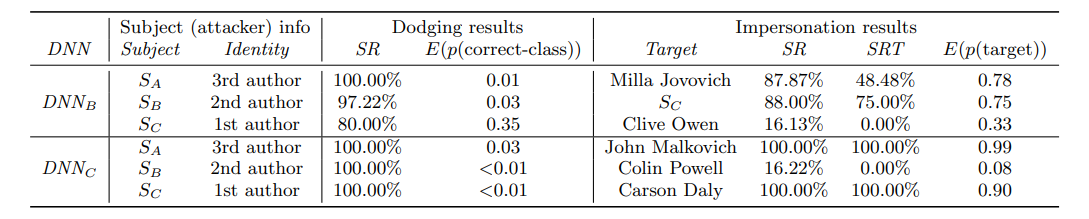
\includegraphics[scale=0.5]{Images/real-world-attack.png}
  \caption{Physical realizability attacks results, SR stands for \textit{success rare} STR stands for \textit{success rate when minimum threshold is used}, $S_A$ is Mahmood Sharif, $S_B$ is Sruti Bhagavatula $S_C$ is Lujo Bauer [2]}
  \label{figurelabel}
\end{figure}




